\documentclass[11pt,a4paper]{article}
\usepackage{amsmath,amssymb,amsfonts,url}
\usepackage{xcolor}
\usepackage[margin=2cm]{geometry}
\usepackage[T1]{fontenc}
\usepackage{ pifont}
\usepackage{multicol}
\usepackage{ulem}
\usepackage{todonotes}   %[disable] option
\allowdisplaybreaks

\renewcommand{\rmdefault}{phv}

\usepackage{pgfgantt}
\newcommand\textganttbar[4]{%
    \ganttbar{#1}{#3}{#4}
    \ganttbar[inline]{#2}{#3}{#4}
}

% ----------------------------------------------------------------
\vfuzz2pt % Don't report over-full v-boxes if over-edge is small
\hfuzz2pt % Don't report over-full h-boxes if over-edge is small

% Hilary's addition to make a compact article and use latex section commands
% make list and enumerate more compact
\usepackage{tweaklist}
\renewcommand{\itemhook}
{
    \setlength{\topsep}{3pt}
    \setlength{\parskip}{0pt}
    \setlength{\parsep}{0pt}
    \setlength{\partopsep}{0pt}
    \setlength{\itemsep}{0pt}
    \setlength{\labelwidth}{10pt}
    \setlength{\leftmargin}{\labelwidth}
}

\renewcommand{\enumhook}
{
    \setlength{\topsep}{3pt}
    \setlength{\parskip}{0pt}
    \setlength{\parsep}{0pt}
    \setlength{\partopsep}{0pt}
    \setlength{\itemsep}{3pt}
    \setlength{\labelwidth}{10pt}
    \setlength{\leftmargin}{\labelwidth}
}

\renewcommand{\deschook}
{
    \setlength{\topsep}{3pt}
    \setlength{\parskip}{0pt}
    \setlength{\parsep}{0pt}
    \setlength{\partopsep}{0pt}
    \setlength{\itemsep}{0pt}
    \setlength{\labelwidth}{0pt}
    \setlength{\leftmargin}{\labelwidth}
}

% Compact sections and parts
\makeatletter
\def\@part[#1]#2
{%
    \refstepcounter{part}%
    {%
        \parindent \z@ \raggedright \interlinepenalty \@M
        \normalfont \Large\bfseries\raggedright
        \partname\nobreakspace\thepart : \nobreakspace #2 %\markboth{}{}\par
    }%
    \nobreak \vskip 1.3ex \@afterheading%
}
\renewcommand\section
{%
    \@startsection {section}{1}{\z@}{-1ex \@plus -0.5ex \@minus -.1ex}%
   {0.5ex \@plus.1ex}{\large\bfseries\raggedright}%
}
\renewcommand\subsection%
{%
    \@startsection {subsection}{1}{\z@}{-1ex \@plus -0.5ex \@minus-.1ex}%
   {0.5ex \@plus .1ex}{\normalfont\bfseries\raggedright}%
}
\renewcommand\subsubsection%
{%
    \@startsection {subsubsection}{1}{\z@}{-0.5ex \@plus -1ex \@minus -.2ex}%
   {0.1ex \@plus .1ex}{\normalfont\bfseries\raggedright}%
}
\renewcommand\paragraph{\@startsection{paragraph}{4}{\z@}%
                                    {0.5ex \@plus0.5ex \@minus.1ex}%
                                    {-0.5em}%
                                    {\normalfont\normalsize\bfseries}}

% subsubsections are actually work packages
\renewcommand{\thesubsubsection}{WP\arabic{subsubsection}}% \hspace{-1em}}
\newcommand\workPackage{\@startsection{subsubsection}{3}{\z@}%
                       {-1ex \@plus -0.5ex \@minus -.1ex}%
                       {0.5ex \@plus .1ex}{\normalfont\bf\raggedright}}

\setcounter{secnumdepth}{5}

% paragraphs are sub work packages
\renewcommand{\theparagraph}{WP\arabic{subsubsection}\alph{paragraph}}%
\newcommand\subworkPackage{\@startsection{paragraph}{4}{\z@}%
                                    {0.5ex \@plus0.5ex \@minus.1ex}%
                                    {-0.5em}%
                                    {\normalfont\normalsize\bfseries}}

\def\@maketitle
{%
  \begin{center}%
  \let \footnote \thanks
    {\large\bf \@title \par}%
    \vskip 0.5em%
    {\normalfont
      \lineskip 1em%
      \begin{tabular}[t]{c}%
        \@author
      \end{tabular}\par}%
    \vskip 0.5em%
    {\large \@date}%
  \end{center}%
  \vskip -2.5em
  \par
  \vskip -1.5em
}
% Reduce the spacing around equations
\AtBeginDocument{%
 \abovedisplayskip=6pt plus 6pt minus 4pt
 \belowdisplayskip=6pt plus 6pt minus 3pt
 \abovedisplayshortskip=0pt plus 3pt
 \belowdisplayshortskip=7pt plus 3pt minus 4pt
}
\setlength{\jot}{0pt}% Inter-equation spacing
\makeatother

% Bibliography stuff
%\usepackage[square,sort&compress,numbers,super]{natbib}
\usepackage[round,sort&compress]{natbib}
%\usepackage[style=authoryear,citetracker,backref, backend=biber]{biblatex}

\setlength{\bibsep}{0pt}
\setlength{\bibhang}{6pt}

% modification to natbib to remove margin
\makeatletter
\renewcommand\NAT@bibsetnum[1]{\settowidth\labelwidth{\@biblabel{#1}}%
%   \setlength{\leftmargin}{\labelwidth}\addtolength{\leftmargin}{\labelsep}%
   \setlength{\leftmargin}{0pt}\addtolength{\leftmargin}{0pt}%
   \setlength{\itemsep}{\bibsep}\setlength{\parsep}{\z@}%
   \setlength{\itemindent}{\bibindent}%
   \ifNAT@openbib
     \addtolength{\leftmargin}{\bibindent}%
     \setlength{\itemindent}{-\bibindent}%
     \setlength{\listparindent}{\itemindent}%
     \setlength{\parsep}{0pt}%
   \fi
}
\makeatother

\usepackage[T1]{fontenc}
\usepackage{pgfgantt, pifont}
\usepackage{multicol}
\usepackage{todonotes,ulem}
\usepackage{color}

\renewcommand{\rmdefault}{phv}

\begin{document}

\title{Case For Support \\ \Large
Multi-fluid modelling of convection
}
\author{Hilary Weller \and Georgios Efstathiou \and John Thuburn \and William McIntyre \and Daniel Shipley}
\date{}
\maketitle

\part{Track Record}

\paragraph*{Dr Hilary Weller (Reading)} has been the lead PI on three NERC grants on atmospheric modelling, a PI on both phases of the Met Office/NERC/STFC UK Dynamical Core project ``Gung-Ho'', to design and build the next Met Office dynamical core and a Co-I on both phases of the NERC/Met Office Paracon projects to improve the modelling of convection in atmospheric models.

Dr Weller has had successful collaborations with Met Office staff, including creating and analysing long time step transport schemes \cite[]{CWPS17,SWMD17} and finding optimal coupling between fast and slow processes \cite[][]{WLW13}. She led pioneering work analysing numerical methods for quasi-uniform grids of the sphere \cite[e.g.][]{WWF09,Wel12,WTC12} and proposed improvements in modelling flow over orography \cite[]{WS14}. 

Before working on numerical methods, Dr Weller worked on tropical meteorology \cite[e.g.][]{LGWS09} which kindled her interest in atmospheric convection. She has combined her applied meteorology experience with her numerical modelling expertise, proposing, with Prof. Thuburn, the use of multi-fluid modelling for representing subgrid-scale convection \cite[]{TWV+18} and creating the first numerical method to solve these equations \cite[]{WM19}. \cite{WMS20} demonstrates a skillful representation of sub-grid dry convection using a multi-fluid model.

\paragraph*{Dr Georgios Efstathiou (Exeter)} is a NERC Independent Research Fellow working on grey-zone turbulence modelling. He has over 15 years of experience in research on the modelling of
atmospheric processes at various scales, from turbulent motions in the boundary layer
to heavy precipitation synoptic systems. An overarching theme is understanding the
connections between atmospheric scales with the aim to improve high-resolution
numerical weather prediction. He has conducted many Large Eddy Simulation (LES) studies and used LES to identify 
the characteristics of the boundary-layer grey zone \citep[e.g.][]{efstathiou2015}
and develop parameterisations suitable for sub-kilometre, very high-resolution models 
\citep{efstathiou2016}. One of his main contributions in grey zone 
studies was the extension of dynamic sub-grid models from the LES to the grey zone region 
providing adaptive and scale dependent turbulence length scales for sub-grid models 
\citep{efstathiou2018,efstathiou2019a}. As part of the NERC/Met Office ParaCon 
project he has developed a novel method to identify updrafts in convective flows 
by optimising the multi-fluid decomposition of the atmosphere \citep{ETB20}.

\paragraph*{Prof. John Thuburn (Exeter)} holds a Chair in Geophysical Fluid Dynamics at the University of Exeter, jointly
funded by the Met Office under the Met Office Academic Partnership.
Since 2000 he has collaborated closely with the Met Office on numerical methods for their
weather and climate models. He made important contributions to the development of the
ENDGame dynamical core \cite[e.g.][]{WSW+14}, which is now a major operational success.
% Could drop the next two sentences
Since 2011 he has collaborated with the Met Office and other UK academic partners on the ``Gung-Ho''
project to develop a future dynamical core suitable for massively parallel computer
architectures. An important theme is to capture key aspects of accuracy related to balance and
conservation on non-traditional grids \cite[e.g.][]{TC15}.

The coupling of physical parameterisations and subgrid models to resolved dynamics is often
particularly subtle because the coupling occurs via marginally resolved and imperfectly
represented scales. Prof.\ Thuburn has contributed to understanding these numerical aspects
of physics-dynamics coupling in the context of quasi-two-dimensional turbulent cascades \cite[e.g.][]{TKW14} and boundary layer parameterisations \cite[]{HTW13a}.
Most relevant for the present proposal is that,
together with co-authors, he developed the mathematical framework for the multi-fluid
approach \citep[][]{TWV+18}, analysed the conservation and normal mode properties
of the unparameterised multi-fluid equations \citep[][]{TV18}, and demonstrated
a proof of concept for a single-column model of the dry convective boundary-layer \citep[][]{TEB19}.


\section*{Institutions}

\paragraph*{The University of Reading Meteorology department} is one of the largest of its kind in Europe with 50 academic staff, 20 senior research staff and fellowship holders, around 90 postdocs and around 70 PhD students. In the 2014 Research Excellence Framework (REF), 86\% of their research was graded as world leading or internationally excellent. Their ``research power'' places them 3rd in the country in Earth Systems and Environmental Science, and the impact of their research was rated 9th highest in the country. The University is a formal Academic Partner of the Met Office and hosts about 20 Met Office scientists. The Reading PDRA will attend Mesoscale group meetings and weekly seminars on atmosphere and ocean science.

\paragraph*{The Department of Mathematics at the University of Exeter} includes the Geophysical and Astrophysical Fluid Dynamics and Exeter Climate Systems research groups, who between them have over~50 staff and over~40 PhD students researching topics related to weather, climate, and modelling. Both groups have excellent track records of collaboration with the Met Office. In the 2014 REF, for UoA 10 (Mathematical Sciences) 83\% of their research was assessed as world leading (4*) or internationally excellent (3*), while for UoA~7 (Earth Systems and Environmental Sciences) 89\% of their research was assessed as 4* or 3*.

\paragraph*{The Met Office} is a world leader in weather forecasting and climate prediction, and their atmospheric model is used by many operational centres (for example, the Australian Bureau of Meteorology). The convection parameterisation group, led by Dr Alison Stirling, publishes widely about their research on aspects of convection, weather prediction and parameterisation. They have just developed a new flexible convection scheme called CoMorph, which will be the basis for future convection developments at the Met Office. Alison's group contributes to ensuring that the Met Office model maintains its high skill and the Met Office maintains its international reputation in numerical weather prediction, climate projection and research. 

\input{trackRecord.bbl}

\newpage

\part{Research Proposal}

{\color{red} My tweaks have made the CFS longer. I have highlighted in red some suggestions for things
to cut, but I didn't want to just hack them out. JT}

{\color{red} Here we seem to be using `closure' instead of `parameterisation'. Usually `closure' means something
slightly different.}

% I have replaced several occurrences of `create'. `Create' is fine in art and cooking when we have a lot
% of freedom. But in science we are constrained by the laws of nature and mathematics, so I prefer
% `develop' or `discover' or something similar.



\section{Motivation and Summary}

The representation of subgrid-scale convection is arguably the weakest aspect of current weather and climate models, leading to unrealistic simulations of monsoons, the diurnal cycle of rainfall, the Madden-Julian Oscillation, and convectively coupled waves  \cite[]{SAB+13,HPB+14}. The representation of the subgrid-scale flow becomes particularly challenging at resolutions where convection is partially resolved -- the grey zone -- as assumptions behind current schemes such as horizontal homogeneity are grossly violated \cite[e.g.][]{GG05}.

Standard convection schemes are based on a simplified %crude
representation of vertical fluxes in terms of a division of the sub-grid flow into separate, homogeneous flows such as updraft, downdraft and environment, with assumptions of small updraft area fraction and horizontally homogeneous quasi-equilbrium, implying no net mass flux and no horizontal transports or propagation. The multi-fluid approach removes these assumptions and has shown promise in single column models. However it is as yet unproven in three-dimensional models and does not address sub-grid variability beyond the multi-fluid division. High-order (or multi-moment) turbulence modelling predicts moments of probability distributions of sub-grid variability. The multi-fluid and multi-moment approaches thus provide two different ways of accounting for sub-grid variability in models, each likely to be most useful in different regimes. Their unification has the potential to work well across a much wider range of regimes, in particular, enabling the construction of a scale-aware model that is applicable at a range of resolutions encompassing the turbulent and convective grey zones.

A three-dimensional multi-fluid, multi-moment model of convection with a seamless transition from fully resolved to grey zone to fully sub-grid convection will be developed by building on existing models and developing improved or completely new parameterisations. We will proceed incrementally, gradually adding complexity to the model formulation and to
the test cases simulated.
A multi-fluid model with a simplified multi-moment representation has already been shown to work well in a single-column, so we will start by simulating fully sub-grid convection in three dimensions using similar parameterisations.
There is room to improve these parameterisations, and improvements and generalisations will certainly be needed
to simulate partially resolved convection. Complete multi-fluid and multi-moment budgets will be diagnosed from
high resolution LES and combined with a toolbox of methods to formulate these improved parameterisations.
The new approach will be evaluated using a suite of equilibrium and non-equilibrium test cases of convective growth and propagation. A key deliverable will be an open source, community model enabling the future research needed to develop the approach towards operational use.

%We will explore the sensitivity of the accuracy to the number of fluids versus the number of moments that are used and which moments should be diagnostic or prognostic (i.e. which level of the Mellor-Yamada hierarchy). We will need to find an appropriate turbulence length scale in a multi-fluid context.

%This proposal will describe a toolbox of methods for finding new closures. High resolution LES will be used to diagnose multi-fluid and multi-moment budgets and evaluate closures. 


\section{Scientific Background}

% I am trying to avoid implying that we `parameterise' convection in the multi-fluid context, because the
% leading order dynamics is meant to be captured by the dycore - this might lead to some convoluted wording
% below, but let's see... JT

%At coarse resolution, convection parameterisation is necessary because, without it, convection is forced to occur at the model grid scale resulting in highly unrealistic behaviour and instability \cite[]{PY15}.
%As supercomputers increase in size, convection is better resolved over larger areas \cite[e.g.][]{GC17} but fully resolving convection over the whole globe is for weather prediction is not likely to ever be achievable \cite[e.g.][]{SSJ+19} so parameterisation will always be needed. 
%Schemes such as mass flux convection remove this instability by re-distributing heat, moisture and momentum in the vertical but not mass \cite[]{Tied89,GR90}. Convection is assumed to be in equilibrium with the large scale so no account is taken of the gradual build-up of convection. Convection in one grid column is assumed to be independent of its neighbours and advection of convective systems is neglected. There have been valuable improvements such as relaxing the quasi-equilibrium assumption \cite[]{PR98,GG05,Par14} and adding stochasticity \cite[]{PC08} but due to the fundamental assumptions in convection parameterisation it has not been possible to create schemes that work well when convection is partially resolved.

Coarse resolution models must represent the effects of subgrid-scale convection, otherwise convection is forced to occur at the model grid scale resulting in highly unrealistic behaviour and possibly model instability \cite[]{PY15}.
As supercomputers increase in power, convection is better resolved over larger areas \cite[e.g.][]{GC17}, but fully resolved convection is not likely to be achieved in the foreseeable future for global weather prediction or routine climate modelling \cite[e.g.][]{SSJ+19}; thus, there is an ongoing need to represent the effects of subgrid-scale convection.
Typical operational convection schemes are built on a set of simplifying approximations:
heat, moisture and momentum are re-distributed in the vertical, but not mass \cite[]{Tied89,GR90}; convection is assumed to be in equilibrium with the large scale so limited account is taken of convective memory and the gradual build-up of convection; convection in one grid column is assumed to be independent of its neighbours and advection of convective systems is neglected. These simplifying approximations are believed to limit the accuracy and physical fidelity of
convection in weather and climate models. Despite recent valuable improvements, such as relaxing the quasi-equilibrium assumption \cite[]{PR98,GG05,Par14} and adding stochasticity \cite[]{PC08}, it has not been possible to develop schemes that work well when convection is partially resolved.

\cite{TWV+18} proposed a new approach --- multi-fluid modelling of convection --- in which convective updrafts, downdrafts and the stable environment are modelled as distinct fluids with separate, but consistent, momentum, continuity, energy and moisture transport equations. The fluids interact via entrainment, detrainment and pressure terms. 
The leading-order dynamics of convection, including non-equilibrium effects, net mass transport, and other horizontal and vertical transports, is explicitly described by these equations, allowing them to be represented by
an extended numerical model dynamical core. Although some processes must still be parameterised, including entrainment,
detrainment, and small-scale turbulent fluxes, these are far fewer than with a traditional convection scheme.
The multi-fluid approach has similarities with the extended EDMF scheme of \cite{TKP+18} who added time derivatives to the EDMF equations.
%Multi-fluid modelling needs some of the same closures as mass-flux parameterisations, such as entrainment and detrainment, but it does away with trigger functions and cloud base mass fluxes, representing those instead as a form of entrainment.
{\color{red} There have been other attempts to include net mass transport by convection \cite[]{KB08,MB19} by modifying existing models, but in a way that is unlikely to work in the grey zone since they do not have numerically stable coupling between the updraft velocity and the pressure.}

{\color{red} The idea of two fluid partitions, each with simple univariate or bivariate Gaussian distributions of sub-grid variability, was used by \cite{GLC02} and forms the basis of the CLUBB parameterisation. However, specifying the parameters in such distributions requires knowledge of (or assumptions about) many high-order moments; multi-fluids each with first or second-order moment equations provides potentially a simpler but more powerful approach.}


% Much work on parameterising turbulence in the atmosphere has focused on the boundary layer. Most relevant to this project is the \citet{mellor1973,mellor1974,mellor1982} MY hierarchy of turbulence closure models. The continuous governing equations were ensemble averaged and manipulated to obtain prognostic equations for all second-order moments such as turbulent kinetic energy (TKE) and subgrid-scale heat fluxes.


Mass flux convection schemes focus on representing the transport due to subgrid-scale coherent structures such as
updrafts. An alternative approach to representing subgrid-scale transports is to solve prognostic or diagnostic
equations for a range of second-order moments. This multi-moment approach is most commonly used for the
boundary layer, and is exemplified by the \citet{mellor1973,mellor1974,mellor1982} MY hierarchy of turbulence
closure models.
There are several reasons for expecting a unification of the multi-fluid and multi-moment approaches to enable
significant advances. It would avoid an artificial separation of boundary layer and convection schemes.
It would enable multi-moment information to be used in the multi-fluid parameterised terms, particularly
entrainment and detrainment. It would enable upgradient turbulent fluxes, such as the fallback of thermals
overshooting the boundary layer inversion, to be represented. Most importantly, it would provide a framework
with the potential to work smoothly across the grey zone from fully resolved to fully sub-grid convection.

We have derived the governing equations for the multi-fluid analogue of the MY hierarchy, but there remain
some key questions, which we aim to investigate. Which combination of multiple fluids and multiple moments
most efficiently describes the sub-grid processes, and does the answer depend on flow regime or model resolution?
How can multi-moment information be best used to inform multi-fluid entrainment and detrainment terms?
How must tuneable coefficients in the MY system, e.g.\ in defining turbulent length scales, be modified
for the multi-fluid case?

Existing parameterisations of entrainment and detainment, and eddy diffusive representation of small-scale turbulent
fluxes, will provide a valuable starting point for the proposed work, and we have had some success with them in
single column models. However, further work is needed to adapt these parameterisations for three-dimensional models,
and especially to formulate the gridscale-dependence that will enable them to work seamlessly across the grey zone.
Discovering quantitatively and causally correct parameterisations is difficult when processes are complex, as in moist convection. Traditionally, progress has been made by combining physical and fluid dynamical understanding with
analysis of detailed process models [and this will remain our primary approach?]. Now, however, 
automated techniques for discovering relationships in the data are rapidly advancing, and 
there are terabytes of convection resolving simulations available. Machine learning with neural networks may be able to discover processes from high resolution data that have not been observed \cite[e.g.][]{ogorman2018}. However, due to their lack of physical basis, neural networks may not be able to extrapolate beyond the range of their training data to new situations such as global warming. An alternative, which enables finding closed-form parameterisations, is the relevance vector machine \cite[e.g.][]{tipping2001}. This uses a sparse Bayesian regression to discover which combination of resolved variables best reproduces a desired subgrid term diagnosed from a high-resolution simulation. This results in a directly interpretable parameterisation and has been used to suggest a successful scale-aware parameterisation for ocean mesoscale eddies \cite[]{zanna2020}.


\section{More detail on Multi-fluid Modelling of Convection}
\label{sec:mf}

The multi-fluid, dry Boussinesq Navier-Stokes equations \cite[approximated by][]{WMS20} are:
\begin{eqnarray}
\frac{\partial\sigma_{i}}{\partial t}+\nabla\cdot(\sigma_{i}\mathbf{u}_{i}) & = & {\textstyle\sum}_{j\ne i}\left\{ M_{ji}-M{}_{ij}\right\} \label{eq:sigma}\\
\frac{D_{i}\mathbf{u}_{i}}{Dt}+\nabla P_{i} & = & b_{i}\mathbf{k}+\nabla\cdot\left( \nu_i\nabla\mathbf{u}_{i}\right)+\frac{1}{\sigma_{i}}{\textstyle\sum}_{j\ne i}\left\{ M_{ji}\left(\mathbf{u}_{ji}^{T}-\mathbf{u}_{i}\right)-M_{ij}\left(\mathbf{u}_{ij}^{T}-\mathbf{u}_{i}\right)\right\} \label{eq:mom}\\
\frac{D_{i}b_{i}}{Dt} & = & \nabla\cdot \left(\alpha_i \nabla b_{i}\right)+\frac{1}{\sigma_{i}}{\textstyle\sum}_{j\ne i}\left\{ M_{ji}\left(b_{ji}^{T}-b_{i}\right)-M_{ij}\left(b_{ij}^{T}-b_{i}\right)\right\} \label{eq:b}\\
{\textstyle\sum}_{i}\nabla\cdot\sigma_{i}\mathbf{u}_{i} & = & 0\label{eq:divFree}\\
{\textstyle\sum}_{i}\sigma_{i} & = & 1.\label{eq:sumOne}
\end{eqnarray}
where $\sigma_i$, $\mathbf{u}_i$, $b_i$ and $P_i$ are the volume fraction, velocity, buoyancy and pressure of fluid $i$. Representing moist convection also needs transport equations for moisture in each fluid and a latent heating term in the buoyancy equation. $M_{ij}$ is the mass transfer rate from fluid $i$ to $j$, which is equivalent to entrainment and detrainment. $\mathbf{u}_{ij}^T$ is the mean velocity of the fluid that is transferred from $i$ to $j$ and $b_{ij}^T$ is the mean buoyancy of the fluid that is transferred. The diffusion terms $\nabla\cdot\left( \nu_i\nabla\mathbf{u}_{i}\right)$ and $\nabla\cdot \left(\alpha_i \nabla b_{i}\right)$ are low-order approximations of subgrid-scale fluxes that occur because each fluid is not uniform at sub-grid scales, with $\nu_i$ and $\alpha_i$ being effective turbulent diffusivities. Higher-order turbulence models predict or diagnose turbulent fluxes rather than representing with a turbulent diffusivity.

{\color{red}
[I would be inclined to follow Dan's suggestion and replace the `diffusion' terms by div of stress tensor and buoyancy flux, especially as the stress tensor should probably be symmetric and trace free.]}

These equations can represent subgrid-scale convection if, for example, fluid 0 is the stable environment, fluid 1 is updrafts and fluid 2 is downdrafts. In order to initialise a multi-fluid model, high resolution data must be partitioned into separate fluids and then averaged onto the (coarser) model grid---this is conditional averaging. The same approach is needed to evaluate the multi-fluid model and to diagnose subgrid-scale fluxes from high resolution data. Techniques such as the optimisation of resolved fluxes \cite[]{ETB20} can be used to define the fluid partitions for the conditional averaging.

For the multi-fluid equations to represent subgrid-scale convection, further closures are needed:\hspace{-1in}
\begin{itemize}
\item Mass transfers between fluids, $M_{ij}$, to represent entrainment and detrainment.
\item The mean buoyancy, moisture and momentum of the fluid that is transferred, $b_{ij}^T$, $q_{ij}^T$ and $\mathbf{u}_{ij}^T$. 
\item Pressure differences between fluids.
\item Subgrid-scale fluxes for each fluid and their interactions. These can be parametrized directly as down-gradient diffusion with turbulent diffusivities of buoyancy, moisture and momentum, or predicted by a multi-fluid extension of the prognostic multi-moment equations.

\end{itemize}
{\color{red} [This is repeating stuff that is now said elsewhere.]
Closures such as entrainment and detrainment rates and turbulent diffusivities from conventional parameterisations can be used with the multi-fluid equations. Complete closure sets specific to multi-fluid modelling have been developed \cite[]{WMS20,TEB19} and proved successful in single-column modelling. We therefore have good starting points for closing the multi-fluid equations but none have yet been shown to work in three dimensions or in the grey zone. }


\section{Relationship with ParaCon}

The poor state of convection parameterisation was the motivation for the \pounds 10M joint NERC, Met Office ParaCon project, which aims to make a ``step change in our ability to predict weather and climate impacts'' by improving parameterisation suitable for existing dynamical cores. This project will use some ParaCon outcomes:
\begin{enumerate}
\item The flexible convection parameterisation scheme CoMorph has been developed for use with the Met Office Unified Model (UM). CoMorph includes new closures for entrainment and detrainment.

\item The MONC LES model was developed and used to produce simulations of convection archetypes. Simulations of the dry and moist convective boundary layer, BOMEX shallow cumuli over the tropical ocean \cite[]{HR73}, radiative-convective equilibrium (RCE), diurnal cycles of deep convection, the shallow cumulus ARM case \cite[]{BCC+02} and the transition from shallow to deep LBA case \cite[]{BFGB02} are available at multiple resolutions.

\item A method of partitioning the atmosphere into coherent thermal structures and their environment was developed \cite[]{ETB20} based on maximising the transport by the mean velocity of each fluid.

\item The Mellor-Yamada closures have been extended to the grey zone and implemented in the UM.

\item A moist, two-fluid, single column model was developed using a variety of entrainment/detrainment closures dependent on turbulent kinetic energy, vertical velocity convergence and atmospheric instability. This is able to reproduce the updraft area fraction ($\sigma_1$) and cloud properties of the ARM case \cite[]{BCC+02} (fig \ref{fig:clouds}). 

\begin{figure}
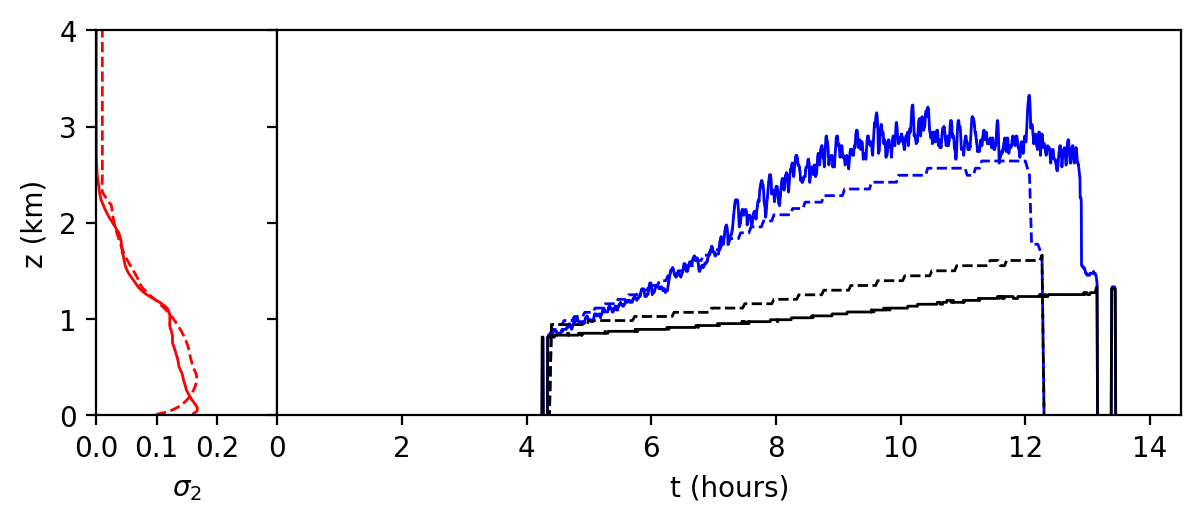
\includegraphics[width=\linewidth]{exeterScm.png}
\caption{Left: the updraft fraction from the large eddy simulation (solid) and the two-fluid single-column model (dashed) at nine hours. Right: The cloud base (black) and cloud top (blue) for the ARM test case. Large eddy simulation (solid) and two-fluid (dashed).}
\label{fig:clouds}
\end{figure}

\item A multi-fluid analogue of the Mellor-Yamada hierarchy was derived including second-moment equations for each fluid type. All of the terms in the original Mellor-Yamada formulation have analogues in the multi-fluid version. There are new terms accounting for transfers between fluids (i.e.\ entrainment and detrainment) and  terms that account for subgrid-scale pressure fluctuations.

\item Fully compressible multi-fluid models with simplified moist physics were developed. MultiFluidAtmosFOAM is a three-dimensional model written using the flexible, parallel modelling framework OpenFOAM, enabling focus on the equations and algorithms rather than the spatial discretisation. {\color{red} Isn't that `job done' then? What is
left to do?}

\end{enumerate}

The multi-fluid approach is not a conventional stand-alone parameterisation that can be called from an existing dynamical core; in contrast to the traditional distinction between `dynamics' and parameterised `physics', it
considers the leading-order dynamics of convection to be part of the `dynamics'. Consequently,
it requires a bottom-up re-development of the model formulation. For this reason, the development of the multi-fluid approach was always expected to extend beyond the end of ParaCon. In this project we will build on the progress made under ParaCon in developing both the multi-fluid approach (basic formulation, stable numerical solutions, sub-grid closures, and single column demonstrations) and the multi-moment turbulence approach by bringing them together.

\section{Proposed Research}

\subsection{Objectives}

The over-arching aim is carry out underpinning research in order to develop a three-dimensional multi-fluid model of the atmosphere that is accurate across a range of convection resolving to subgrid-convection resolutions with three essential, minimum properties:

\begin{enumerate}\renewcommand{\theenumi}{\alph{enumi}}
\item When convection is well resolved, the solutions are identical to a single fluid model.
\item When convection is fully sub-grid, the solutions are at least as accurate as a dynamical core with a conventional parameterisation.
\item When convection is partially resolved, the solutions are more accurate than a single-fluid model with no parameterisation and more accurate than the multi-fluid model at coarse resolution.
\end{enumerate}

We plan to meet these aims via these specific objectives:

{\color{red} Should these objectives match up with the work packages? They half do. Also, it feels like there's a
bit of an artificial separation between single moment and multi-moment, and between development and evaluation.
And a mismatch between objective 6 and WP7.}

\begin{enumerate}
\item\label{it:model} Develop a flexible, three-dimensional multi-fluid, multi-moment model of the atmosphere including three phases of moisture. This objective does not include finding optimal closures.

\item\label{it:budgets} Calculate budgets of subgrid-scale fluxes from LES data in order to diagnose the values of entrainment and detrainment and other closures.

\item Using the the techniques described in section \ref{sec:tools}, find and test suitable closures so that the single-moment, multi-fluid model represents under-resolved dry and moist convection using simple models of turbulent fluxes.

\item Combine multi-fluid and Mellor-Yamada modelling to develop a  multi-fluid, multi-moment model for turbulent convection including consistent interactions between moments and fluids and closures for unknown correlations between moments.

\item Investigate which combination of multiple fluids and multiple moments most efficiently captures subgrid-scale
variability and transport for different types of convection and at different resolutions.

\item Evaluate using a hierarchy of convective cases from the Paracon project.

\item Deliver an open access, well documented, parallel, multi-fluid model of the atmosphere with well documented performance at representing convection across scales.
\end{enumerate}

\subsection{Work Packages}
\label{sec:WPs}

\workPackage{Flexible Modelling Framework (Reading, 6 months) \label{WP:model0}}

Using the OpenFOAM flexible modelling framework and using the code developed during Paracon we will develop multiFluidAtmosFOAM, a three-dimensional multi-fluid, multi-moment including moisture and some simple transfer terms and closures. This work will involve software testing and testing of exact properties such as conservation but will not aim to represent convection accurately. Combining code from Reading and Exeter will enable us to benchmark against the existing codes. All code will be version controlled and uploaded to a public \url{github.com} repository. A model description paper will be submitted to Geoscientific Model Development. This model will be suitable for carrying out the research in the rest of the project. 

Some of the multi-fluid code developed during Paracon was fully compressible and some was Boussinesq. We do not need to include the complexities of full compressibility in multiFluidAtmosFOAM as this is not central to convection and the LES model that we are comparing with is anelastic. 

\workPackage{LES Budgets (Exeter, 9 months) \label{WP:LESbudgets}}

We will carry out detailed diagnostics of the LES data created during ParaCon, computing complete budgets for all second-moment quantities for the cases of a single fluid, two fluids (updraft and environment), and, for LBA, three fluids (updraft, downdraft, and environment).
We will decompose the flow into updrafts and their environment using the optimal decomposition developed during Paracon and extend this to diagnose coherent downdrafts. The budgets will be calculated for a range of horizontal filter scales, from a global horizontal average down to scales comparable to the cloud width and boundary layer depth. From the LES we can calculate the size but not the form of the closures.

\workPackage{Multi-fluid modelling of dry convection (Reading, 6 months) \label{WP:dryMF}}

An important aspect of our approach is to find closures within the simplest possible framework to avoid multiple competing influences contaminating the results. Hence we will ensure that the entrainment and detrainment and pressure differences between fluids are correctly modelled for dry convection first using the tools described in section \ref{sec:tools} and using Paracon data.

We will simulate the dry convective boundary layer (CBL) with two fluids and using the same turbulent moments as were effective in the single column framework (fig \ref{fig:clouds}). We will evaluate and develop closures first in the fully parameterised regime and then at different resolutions of the grey-zone.

\workPackage{Multi-fluid modelling of moist convection (Reading, 9 months) \label{WP:moistMF}}

We will add three phases of water with simple microphysics and explore to what extent we can parameterise shallow and deep convection cases from the hierarchy with two or three fluids but with existing models of turbulent fluxes. Closures will be sought that that work through the grey zone with the limiting cases of fully parameterised and fully resolved convection.

\workPackage{Multi-moment, multi-fluid modelling of dry convection (Exeter, 9 months) \label{WP:YMdry}}

The different levels of closure model proposed by Mellor and Yamada are based on neglecting transience, advection, and third-order turbulent transport in various second-moment equations. Using the budgets calculated in \ref{WP:LESbudgets}, we will test the validity of making analogous approximations for different numbers of fluids and for different filter scales in the boundary layer. The diagnosed distributions of third-order terms, pressure-correlation terms, and dissipation terms will be compared with the models proposed by Mellor and Yamada (and subsequent authors). The length scales required to optimise the multi-fluid Mellor-Yamada scheme will be compared for different filter scales and different numbers of fluids, paying particular attention to the grey zone. We will also use the information provided by the moments to better parameterise entrainment and detrainment using methods from the toolbox (below).

\workPackage{Multi-moment, multi-fluid modelling of moist convection (Exeter, 12 months) \label{WP:YMmoist}}

Building on the LES simulations and the single-column, multi-fluid, multi-moment simulation of the ARM test case (see fig \ref{fig:clouds}), we will simulate this test case with the three-dimensional multi-fluid, multi-moment model at coarse resolution with the same closures as the single-column model.  We will next increase the resolution into the grey zone where existing parameterisations may not work so well. We will explore whether additional moments or a third fluid are needed in order to best represent the sinking of overshooting thermals. 

We will simulate a radiative-convective equilibrium case without aggregation and compare with Paracon LES data. We will check that the equilibrium conditions are not sensitive to modelling assumptions about the initial conditions and are not resolution dependent through the grey zone.


\workPackage{Evaluation \label{WP:evaluate} (Exeter, 6 months, Reading, 9 months)}

The evaluation will use a different test case with different forcings in order to test if the new model is predictive rather than a fit to LES. This will consist of a squall line over flat terrain \cite[]{FM06}. In order to test if we are doing better than a state of the art conventional parameterisation, we will compare with the idealised Met Office UM model using the CoMorph parameterisation at coarse resolution using the same simplified microphysics. Squall lines are known to be challenging for standard convection parameterisations \cite[e.g.][]{LCD+08} due to the lack of propagation of convection and the lack of mass transport by convection. We will evaluate sensitivity to resolution through the grey zone. 

We will compare different versions of multiFluidAtmosFOAM with different closures, different numbers of fluids and different moments in order to find how many terms and how many prognostic equations need to be retained. 

\workPackage{A community turbulent multi-fluids model \label{WP:model} (Reading, 6 months)}

MultiFluidAtmosFOAM will be developed throughout the project. The final anelastic version will:
\begin{enumerate}
\item solve for one, two or three fluids;
\item include prognostic equations for second moment of variables within each fluid;
\item use Cartesian geometry and no orography;
\item include simplified radiation and moist physics, a simplified bottom boundary and no stratosphere;
\item be parallelised using MPI.
\end{enumerate}
We will create documentation and a set of test cases for new users to run. A part II model description paper will be submitted to Geoscientific Model Development.

\subsection{Tools for Finding and Evaluating Closures}
\label{sec:tools}

{\color{red} For me the top of the list would still be the traditional approach of fluid-dynamical understanding
(and physical and mathematical consistency) plus hi-res process modelling to formulate as well as tune
parameterisations. But I guess this includes several of the items below...}


Good candidates exist for closing the multi-fluid, multi-moment equations. The success of this project does not rely completely on finding new closures since the multi-fluid framework may prove beneficial even with existing closures. We have a toolkit for evaluating closures and finding new ones. We will pay particular attention to how relationships between sub-grid terms and resolved variables vary across scales. 

\subsubsection*{Optimise Existing Closures}

From the LES data we will calculate the parameters that optimise existing closures. If optimised parameter values vary only a little between test cases the then existing closure may prove useful.

\subsubsection*{Assumed Multi-fluid Probability Distribution Functions (PDFs)}

Fluid properties can be represented as bi-or tri-Gaussians using the mean and variance of each fluid. From these it is possible to calculate the mass of fluid that crosses a threshold that defines the fluids. This implies a mass transfer (similar to transferring the tails of the distribution). The mean properties of the fluid transferred can also be calculated from the distribution. This approach was explored in the PhD thesis \cite{McIn20} supervised by Weller.

\subsubsection*{Theory of Distributions}

Derivations of multi-fluid equations make use of discontinuous functions to label different regions of the underlying fluid \cite[]{Dopa77,TWV+18}. The terms requiring closure in such an approach depend on derivatives of those discontinuous functions. The theory of distributions (or generalised functions) \cite[]{Schw08} allows for the definition and manipulation of such discontinuous functions and their derivatives. This can be used to derive exact integral expressions for the terms requiring closure. Once conditions are specified to split the flow into multiple fluids, these conditions can be used to compute the closures directly from LES data. We will also use this method to suggest closures by considering simplified flows, and asymptotic approximations of evolution equations. For instance, the integrals can be calculated analytically for the first normal mode of Rayleigh-B\'{e}nard convection  \cite[]{SWCM2x}. This will lead to new physically-based closures for the entrainment and detrainment terms in a multi-fluid model. 

\subsubsection*{Asymptotics}

Candidate closures will be used to simulate various idealised test cases and we will demand:
\begin{enumerate}
\item Term-by-term Galilean invariance.
\item Two initially identical fluids should remain identical when mixed.
\item For any linear term of the multi-fluid equations, summing over all fluids should lead to the equivalent term of the original single-fluid equations.
\item  When convection is fully resolved, two fluids should evolve as one.
\item\label{it:energyTransfer} Closures and numerical methods should not create energy and not create or destroy first moments of primitive variables.
\item\label{it:boundedTransfer} Closures and numerical methods should not create new extrema except where second-order moments provide sources for first-order moments.  Numerical methods to ensure \ref{it:energyTransfer} and \ref{it:boundedTransfer} were derived by \cite{MWH20}.
\item At coarse resolution, a two-fluid model should be more accurate than a single-fluid model at the same resolution. By more accurate we mean that conditional averages are closer to a fully resolved single-fluid model.
\item An initially empty fluid should not influence a non-empty fluid.
\end{enumerate}
Existing convection parameterisations do not have these properties, which can lead to spurious solutions in the grey zone.

Once a set of closures obeys the above constraints, we will evaluate by developing coarse resolution multi-fluid models of LES convection cases developed during Paracon. These will increase in complexity in order to maintain an unambiguous link between additional complexity and model fidelity. They will start as single column, then fully parameterised coarse resolution and finally partially resolved (grey zone). 

\subsubsection*{The Relevance Vector Machine (RVM)}

From the analysis of the LES (\ref{WP:LESbudgets} above) we will be able to calculate exactly the size but not the form of the closure needed to produce correct multi-fluid results. To apply the RVM we will also create a library of resolved variables which the specified subgrid term is conjectured to depend on. The RVM can then be used to discover which combination of resolved variables best reproduces the subgrid terms. This would provide physical insight into how the coherent structures of convection act, and to what extent that interaction can be universally represented.

\section{Potentials for Impact}

{\color{red} This section and the next are brief and weak.}

If we are able to show that multiFluidAtmosFOAM can represent convection more accurately than single-fluid models for a similar computational cost, then multiFluidAtmosFOAM can be further developed to create a more complete model that can be used for weather and climate prediction.

Earlier opportunities for impact will come from our data analysis. The closures that we develop for the multi-fluid equations are likely to be useful for other parameterisations of convection. Collaboration with the Met Office will ensure that useful developments see early operational use. 

\section{Management and Collaboration}

We plan to work as one team across both institutions and will meet together online once a week. Meetings with Met Office will be held four times a year to discuss project progress and plans and to co-ordinate evaluation, comparing with the idealised UM (see letter of support from the Met Office). Insights gained during this project will feed into the Met Office model development.

\section{Risks and Mitigations}

Some of the risks associated with this proposal are generic to modelling: slow code development and uncertainties in the results. These risks are mitigated by the experience of the investigators and researchers and by the flexible and advanced code that has already been developed.

There are some dependencies between work packages; the development and evaluation of closures relies on the LES analysis. However the theoretical work and the single-moment, multi-fluid model development can proceed without the results of the LES analysis. The evaluation relies on the model development work packages.

Multi-fluid modelling cannot be retro-fitted to an existing model as is usually done with convection parameterisations. This means that a whole new model is needed in order to produce a multi-fluid model of convection. This is a big undertaking for operational centres so the biggest risk is that multi-fluid modelling will not be adopted by big modelling centres. We therefore plan to create models with enough functionality to be useful for independent research into convection and parameterisation.

\renewcommand\refname{References (not included in Track Record)}
\input{proposedResearch.bbl}
%\newpage
%\renewcommand\refname{All References (not for submitted copy)}
%\bibliography{Weller,Thuburn,Shipley}
\bibliographystyle{myNat}

\end{document}
